\section{Introduction}
\label{sec:intro}


In computer graphics and vision, achieving realistic renderings for intricate surface materials hinges on accurately describing the interaction of light with the surfaces. This is conventionally conveyed through the modeling and reconstruction of a 4D Bidirectional Reflectance Distribution Function (BRDF), which quantifies the relationship between the incident and outgoing light intensities for a specific material. In this work, we propose a novel generalizable BRDF representation model that can estimate the BRDFs of new materials from highly sparse and unstructured point-based samples \footnote{Point-based samples refer to the BRDF values acquired at specific points on a surface with known viewing and lighting directions.} and compress the densely sampled values into very small latent embeddings.


While there has been prior work that attempts to tackle similar tasks by estimating the free parameters of analytic BRDF functions or the principal components of BRDF functions from images or reflectance measurements, the oversimplified models of the complex BRDF function lead to inaccuracies when predicting real materials, thereby diminishing the realism in renderings~\cite{ngan2005}. Moreover, the process of fitting through nonlinear optimization is inherently unstable, computationally expensive, and prone to local minima, hindering the accurate reconstruction of material appearance~\cite{dupuy2015, guarnera2016}. Measured BRDFs of real-world materials can also be fraught with errors due to equipment limitations, adding to the complexity of the fitting process~\cite{nielsen2015optimal}. 

\begin{figure}
  \centering
   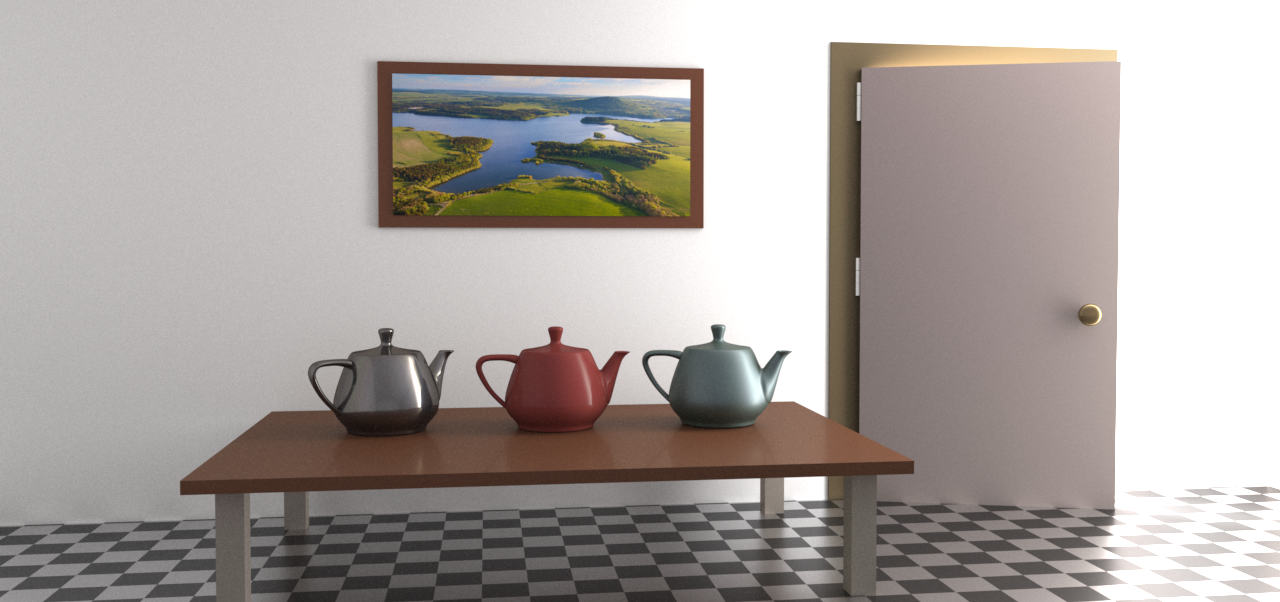
\includegraphics[width=\linewidth]{Chapters/hyperbrdf-figs/teaser_cropped.png}
   \caption{A room scene rendered with our reconstructed materials, including sparse reconstruction (table top and legs, door, door and picture frames, hinge), compression (two teapots on the left, door handle) and BRDF interpolation (right-most teapot). Scene courtesy of Benedikt Bitterli.}
   \label{fig:teaser}
\end{figure}

Recent advances in deep learning have enabled the accurate representation of complex continuous signals (\textit{e.g.} images, surfaces, volumes, materials, \textit{etc.}) using a Neural Field~\cite{sitzmann2020siren, ffn, cnf2023}, \textit{i.e.} a neural network mapping coordinate inputs to sampled values, without compromising model compactness. Consequently, neural fields have gained substantial popularity for representing continuous BRDFs in recent works~\cite{sztrajman2021neural, cnf2023}. However, reconstructing a neural field representation for BRDFs typically requires training the network with a regression loss function to overfit to a single material, which demands dense sampling and extensive computational resources, while being unable to generalize to new materials.

More recently, Generalizable Neural Fields~\cite{rebain2022attention} (GNFs) have emerged as a promising solution to the aforementioned challenges. Rather than overfitting to individual signals, GNFs are designed to learn a generalized mapping, either deterministic or probabilistic, between sampled signals and their full neural field representations in a fashion similar to supervised learning.
The key strategy of GNFs involves conditioning the neural fields with a latent embedding of the signal samples. Popular conditioning mechanisms include concatenated latent vectors~\cite{park2019deepsdf}, hypernetworks~\cite{ha2017hypernetworks}, and attention-based set latent representations~\cite{jiang2021cotr}. Once the conditional neural field is properly learned, reconstruction of the full signal can be achieved at inference time, and even with highly sparse and unstructured samples.


Inspired by GNFs, we propose a novel framework for generalizable neural BRDF representation for both the estimation of unseen materials from sparse and unstructured samples and the compression of measured BRDFs into low-dimensional latent space. In this framework, we employ a multi-layer perceptron (MLP) model as the neural field backbone for BRDF representation, a hyper-network for conditioning, and a set encoder that allows for mapping an arbitrary number of reflectance measurements from arbitrary directions to a compact latent embedding for conditional BRDF generation. 
The built-in nonlinear interpolation capability of the hyper-network also offers robust and adaptable material editing and blending across various sample sizes.


Unlike previous work, our BRDF reconstruction is highly efficient without the need for extensive training to overfit individual materials, while also maintaining state-of-the-art performance in reconstruction accuracy for sample size below 4000; see Figure~\ref{fig:imp_comp_upt}.


In summary, we offer a novel solution for the challenging task of generalizable BRDF modelling with the following key contributions:
\begin{itemize}
    \item{\textbf{Generalizability and Adaptability:} Our methodology ensures robustness and adaptability across varying sample sizes and appearances, making it highly effective for estimating the BRDFs of unseen materials from highly sparse and unstructured sampling. Its adaptability also extends to highly compact representation of BRDFs, overall outperforming the prior state-of-the-art compression method; see Table \ref{table: oursvsnps}.}
    

    \item{\textbf{Realism and Accuracy:}
    Our extensive evaluation demonstrates the superior performance of our approach in reconstructing the BRDFs of 20 test materials from a limited number of samples, ranging from 40 to 4000, outperforming prior methods in terms of appearance modeling and color preservation (by at least 2dB in peak-signal-to-noise ratio and 1 in Delta E).
    }
\end{itemize}


\section{Acquisition Systems}
\label{sec:Acquisition-Systems}
